We consider the Gaussian sequence space model where, for any $s$ in $\N$, we have $Y(s) \sim \mathcal{N}(\phi(s), 1)$ and hence $\phi_{n}(s) \sim \mathcal{N}(\phi(s), n^{-1})$; and $\epsilon(s) \sim \mathcal{N}(\lambda(s), 1)$ and hence $\lambda_{n_{\lambda}}(s) \sim \mathcal{N}(\lambda(s), n_{\lambda}^{-1})$.

We will apply the strategy we just presented to this model, first with $\lambda$ known, then with $\lambda$ estimated.
In both cases, quadratic as well as maximal risk are bounded.

\subsection{Known operator}\label{freq:igssm:kn}
We assume here that we know $\lambda$ and observe the vector of independent random variables $Y^{n}$.
Assume now that for any $s$ in $\N$, we know $\lambda(s) > 0$.
\subsubsection{Shape of the estimator}
First, let us remind that we plan to use an aggregated orthogonal series estimator $\widehat{\theta}^{(\eta)}$, with $\eta$ in $\R_{+}^{\star} \cup \infty$ which form is reminded hereafter.
\begin{de*}
We first define so-called contrast $\Upsilon$ and penalisation $\pen^{\Lambda}$ sequences, which allow us to define weight $\P_{M}^{(\eta)}$ on the nested sieve space (here $(\llbracket 0, m \rrbracket)_{m \in \N}$)
\begin{multline*}
\Upsilon : \mathds{N} \to \R_{+}, \quad m \mapsto \Upsilon(m); \qquad \pen^{\Lambda} : \N \to \R_{-}, \quad m \mapsto \pen^{\Lambda}(m);\\
\P_{M}^{(\eta)} : \N \to \R_{+}, \quad m \mapsto \tfrac{\exp[\eta n (\Upsilon(m) + \pen^{\Lambda}(m))]}{\sum\nolimits_{k = 0}^{n} \exp[\eta n (\Upsilon(k) + \pen^{\Lambda}(k))]} \mathds{1}_{m \leq n}.
\end{multline*}
Notice that letting $\eta$ tend to $\infty$ in the previous definition gives rise to the penalised contrast model selection estimator,
\begin{equation*}
  \tDi:=\argmin\nolimits_{\Di\in\nset{1,\ssY}} \big\{\Upsilon(m) + \penSv\big\}
\end{equation*}
which corresponds to the following weights
\begin{equation*}
  \lim\nolimits_{\rWc\to\infty}\rWe=\dirac[\tDi](\{\Di\})=:\msWe.
\end{equation*}
Here, we will use the following shape for $\Upsilon$ and $\pen^{\Lambda}$, for $\cpen := 84$
\begin{alignat*}{4}
  & \Upsilon(m) && := && \Vert \theta_{n, \overline{m}} \Vert_{l^{2}}^{2};  \quad && \cmiSv := \tfrac{\log^{2}(\Di\miSv \vee(\Di+2))}{\log^{2}(\Di+2)}\geq1;\\
  & \DipenSv && := && \cmiSv \Di \miSv; \quad && \penSv:= \penD.
  \end{alignat*}
  \assEnd
\end{de*}
The family of estimators is hence entirely defined and can be implemented with the data we assume to have at hand in this subsection.

\subsubsection{Oracle optimality}
In a first time we are interested in the quadratic risk for any $\theta^{\circ}$ fixed.
Remind that the strategy we use allows to show that the following sequence is an upper bound for the quadratic risk.
\begin{de*}
Remind that we defined for any $\theta$ in $\Theta$ and $\Di$ in $\N$ the following term $\b_{m}^{2}(\theta) = \Vert \theta_{\underline{m}} \Vert_{l^{2}}/\Vert \theta_{\underline{0}} \Vert_{l^{2}} \leq 1$.
We then define a family of sequences $(\daRa{\Di}{(\xdf)})_{\Di \in \N} := (\daRa{\Di}{(\xdf,\Lambda)})_{\Di \in \N} = [\b_{m}^{2}(\theta^{\circ}) \vee \penSv/\cpen]$ and hence it holds for all $\Di$ in $\nset{1,\ssY}$
    \begin{equation}
      [\Vnormlp{\xdf_{\underline{0}}}^2+\cpen]\daRa{\Di}{(\xdf)}\geq\Vnormlp{\xdf_{\underline{0}}}^2\bias^2(\xdf)\vee\penSv.
      \end{equation}
We intend to prove that the specific choice
\begin{multline*}
\aDi{\ssY}(\xdf):=\argmin\Nset[\Di\in\Nz]{\daRa{\Di}{(\xdf)}}\in\nset{1,\ssY}; \\
\naRa{(\xdf)}:=\naRa{(\xdf,\Lambda)}:=\min\Nset[\Di\in\Nz]{\daRa{\Di}{(\xdf)}}
\end{multline*}
with $\daRa{\aDi{\ssY}}{(\xdf,\Lambda)}=\naRa{(\xdf,\Lambda)}$ defines an upper bound for the convergence rate of the aggregation estimators.
\assEnd
\end{de*}

A direct application of \nref{lmA.1.1} and \nref{lmA.1.2} gives us the following result.
\begin{cor*}
For any $m$ and $n$ in $\N$, we have
\begin{alignat*}{3}
& \E[(\Vert \theta_{n, \overline{m}} - \theta^{\circ}_{\overline{m}} \Vert_{l^{2}}^{2} - 12 \Delta_{\Lambda}(m) n ^{-1})_{+}]&& \leq && 6 \Lambda_{+}(m) n^{-1} \exp[-2 \delta_{\Lambda}(m) m]\\
& \P(\Vert \theta_{n, \overline{m}} - \theta^{\circ}_{\overline{m}} \Vert_{l^{2}}^{2} \geq 12 \Delta_{\Lambda}(m) n ^{-1})&& \leq &&\exp[-2 \delta_{\Lambda}(m) m]\\
& \P(\Vert \theta_{n, \overline{m}} - \theta^{\circ}_{\overline{m}} \Vert_{l^{2}}^{2} \geq 12 \mathfrak{R}_{n}^{m}(\theta^{\circ}, \Lambda))&& \leq &&\exp[-2 \tfrac{\mathfrak{R}_{n}^{m}(\theta^{\circ}, \Lambda) n}{\Lambda_{+}(m)}]
\end{alignat*}
\reEnd
\end{cor*}
Hence, \nref{freq:ge:strat:kn:qu:as} is verified with constants $\cst{1} = 1, \cst{2} = 6, \cst{3} = 2, \cst{4} = 0, \cst{6} = 1, \cst{7} = 2, \cst{9} = 1, \cst{10} = 2$, notice that $\cst{5}$, $\cst{8}$, and $\cst{11}$ are irrelevant here as the corresponding term is not present.
We can hence apply the theorem me presented earlier.

The following theorem is then a direct application of \nref{freq:ge:strat:kn:qu:pnp} and we omit its proof.

\begin{thm}
Consider the penalty sequence $\penSv:=\penD$, $\Di\in\nset{1,n}$, as in \nref{freq:ge:shape:kn:de:pen:oo} with numerical constant $\cpen \geq 84$.
Let $\txdfAg[{\erWe[]}]=\sum_{\Di=1}^{\ssY}\We\txdfPr$ be an aggregation of the orthogonal series estimators, using either aggregation weights $\rWe[]$ as in \eqref{freq:ge:shape:kn:we}, or model selection weights $\msWe[]$ as in \eqref{freq:ge:shape:kn:de:msWe}.
\begin{Liste}[]
\item[{\dgrau\bfseries{(p)}}]Assume there is $K\in\Nz$
  with   $1\geq \bias[{[K-1] }](\xdf)>0$ and $\bias[\Di](\xdf)=0$. For
  $K>0$ let
  $ c_{\xdf}:=\tfrac{\Vnormlp{\xdf_{\underline{0}}}^2+4\cpen}{\Vnormlp{\xdf_{\underline{0}}}^2\bias[{[K-1]}]^2(\xdf)}>1$ and
  $\ssY_{\xdf}:=\gauss{c_{\xdf}\DipenSv[K]}\in\Nz$. If
  $\ssY\in\nset{1,\ssY_{\xdf}}$ then set $\sDi{\ssY}:=\Di_{\cst{3}}\log(\ssY)$, and otherwise if
  $\ssY>\ssY_{\xdf}$ then set
  $\sDi{\ssY}:=\max\{\Di\in\nset{K,\ssY}:\ssY>c_{\xdf}\DipenSv\}$
  where the defining set contains $K$ and thus is not empty.
There is a finite constant $\cst{\xdf,\Lambda}$
given in \eqref{ak:ag:ub:pnp:p7} depending only on $\xdf$ and $\Lambda$ such that for all $n\in\Nz$ holds
\begin{equation}
  \nRi{\txdfAg[{\erWe[]}]}{\xdf,\Lambda}
  % \E\Vnormlp{\txdfAg[{\erWe[]}]-\xdf}^2
  \leq
  \cst{}\Vnormlp{\xdf_{\underline{0}}}^2\big[
  \ssY^{-1}\vee\exp\big(-2\cmiSv[\sDi{\ssY}]\sDi{\ssY}\big)\big]
  + \cst{\xdf,\Lambda}\ssY^{-1}.
\end{equation}
\item[{\dgrau\bfseries{(np)}}] Assume that
  $\bias(\xdf)>0$ for all  $\Di\in\Nz$.
There is a finite finite constant $\cst{\xdf,\Lambda}$ given in
\eqref{ak:ag:ub:pnp:p8} depending only $\xdf$ and $\Lambda$ such that for all
$\ssY\in\Nz$  holds 
 \begin{equation}
   \nRi{\txdfAg[{\erWe[]}]}{\xdf,\Lambda}
   % \E\Vnormlp{\txdfAg[{\erWe[]}]-\xdf}^2
    \leq 
   \cst{}(\Vnormlp{\xdf_{\underline{0}}}^2\vee1)\min_{\Di\in\nset{1,\ssY}}\big[\dRa{\Di}{\xdf,\Lambda}\vee\exp\big(-2\cmiSv\Di\big)\big]\\
   +\cst{\xdf,\Lambda}\ssY^{-1}.
\end{equation}
\end{Liste} 
\reEnd 
\end{thm}

\begin{cor}
  Let $\cpen \geq 84$.
  \begin{Liste}[]
  \item[{\dgrau\bfseries{(p)}}]
    If in addition
    \begin{inparaenum}\item[{{\dgrau\bfseries(A1)}}]
      there is
      $\ssY_{\xdf,\Lambda}\in\Nz$ such that
      $\cmiSv[\sDi{\ssY}]\sDi{\ssY}\geq (\log\ssY)/2$ for all
      $\ssY\geq \ssY_{\xdf,\Lambda}$
    \end{inparaenum}
    holds true, then there is a constant $\cst{\xdf,\Lambda}$ depending
    only on $\xdf$ and $\Lambda$ such that for all $n\in\Nz$ holds
    $\nRi{\txdfAg[{\erWe[]}]}{\xdf,\Lambda} \leq
    \cst{\xdf,\Lambda}\ssY^{-1}$.
  \item[{\dgrau\bfseries{(np)}}]
    If in addition
    \begin{inparaenum}\item[{{\dgrau\bfseries(A2)}}]
      there is  $\ssY_{\xdf,\Lambda}\in\Nz$ such that
      $\aDi{\ssY}(\xdf)\cmSv[\aDi{\ssY}(\xdf)]\geq \vert \log\naRa{(\xdf,\Lambda)} \vert/2 $
      for all $\ssY\geq \ssY_{\xdf,\Lambda}$
    \end{inparaenum}
    holds true, then there is a constant $\cst{\xdf,\Lambda}$ depending
    only on $\xdf$ and $\Lambda$ such that $\nRi{\txdfAg[{\erWe[]}]}{\xdf,\Lambda}
    \leq \cst{\xdf,\Lambda}\naRa{(\xdf,\Lambda)}$ for all $n\in\Nz$ holds true.
  \end{Liste} 
    \reEnd 
\end{cor}

In \nref{fig:freq:igssm:error} we give an illustration of the error of the aggregation estimator with $\eta = 1$, of the oracle projection estimator and of the model selection estimator, in the Gaussian sequence space model in the case of a direct problem, with the same data.

\begin{figure}
  \centering
  \begin{tabular}{@{}c@{}}
    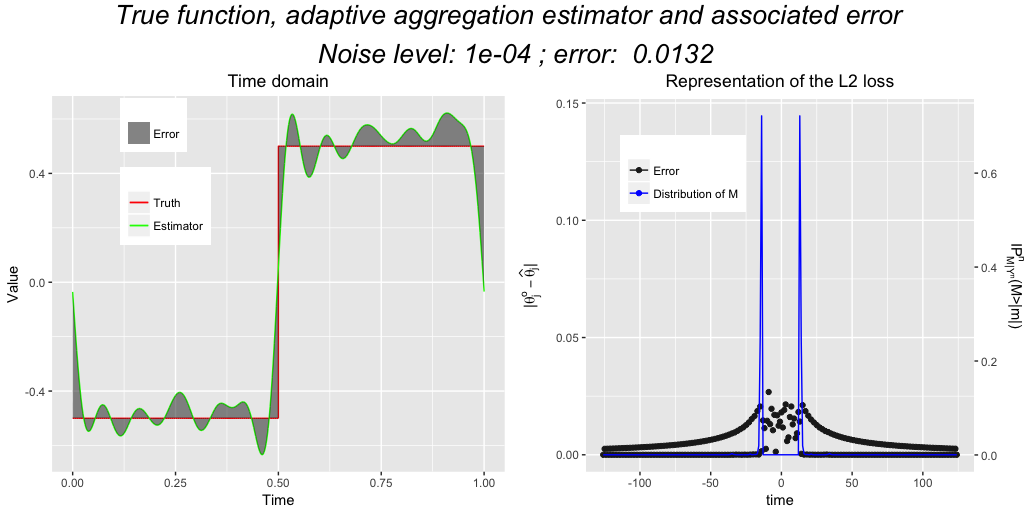
\includegraphics[width=.4\linewidth]{gauss/error/aggregation_error.png} \\[\abovecaptionskip]
  \end{tabular}
  \begin{tabular}{@{}c@{}}
    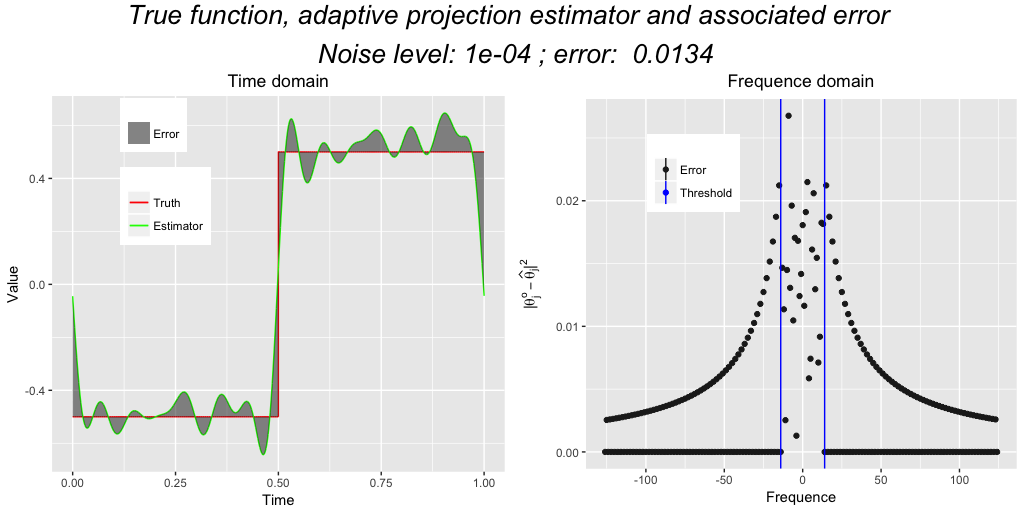
\includegraphics[width=.4\linewidth]{gauss/error/model_selection_error.png} \\[\abovecaptionskip]
  \end{tabular}
  \caption{Error of the aggregation estimator and of the model selection estimator for a fixed dataset}
  \label{fig:freq:igssm:error}
\end{figure}

Replicating the same experiment as in \nref{fig:freq:igssm:error} many times, it allows us to estimate the distribution of the error of each estimator at a fixed value of $n$, which we represent in \nref{fig:freq:igssm:error:mcmc}.

\begin{figure}
  \centering
  \begin{tabular}{@{}c@{}}
    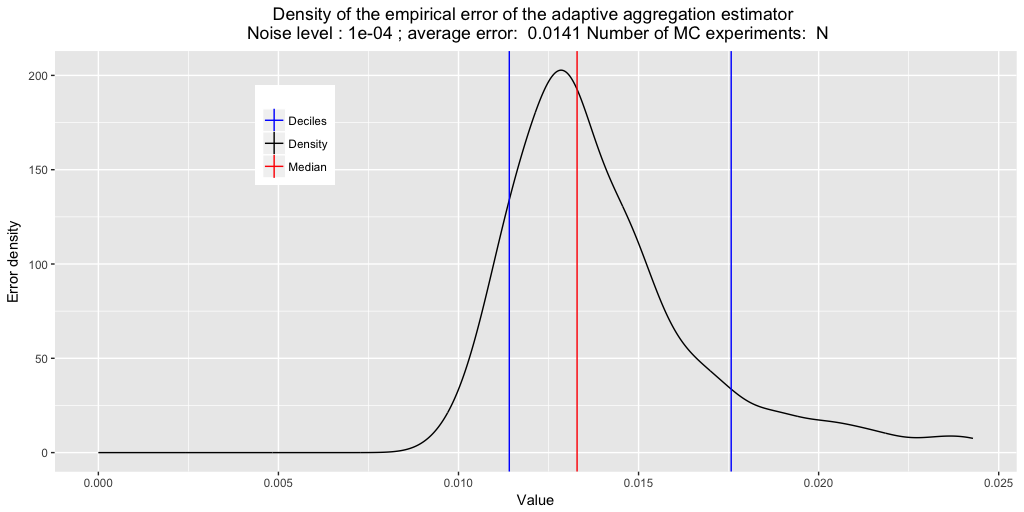
\includegraphics[width=.4\linewidth]{gauss/MCMC/error_aggregation.png} \\[\abovecaptionskip]
  \end{tabular}
  \begin{tabular}{@{}c@{}}
    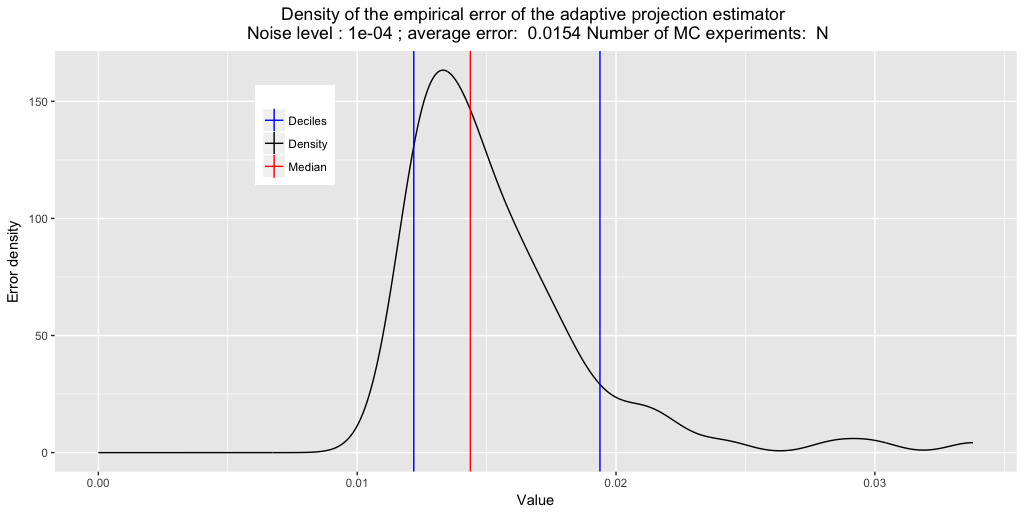
\includegraphics[width=.4\linewidth]{gauss/MCMC/error_model_selection.png} \\[\abovecaptionskip]
  \end{tabular}
  \caption{Kernel estimation of the density of the error for the aggregation estimator and the model selection estimator for a fixed true parameter $\theta^{\circ}$ and noise level $n$}
  \label{fig:freq:igssm:error:mcmc}
\end{figure}

Finally, replicating the experiment of \nref{fig:freq:igssm:error:mcmc} for different values of $n$ we can illustrate the evolution of the risk with $n$, as represented in \nref{fig:freq:igssm:error:evol}.

\begin{figure}
  \centering
  \begin{tabular}{@{}c@{}}
    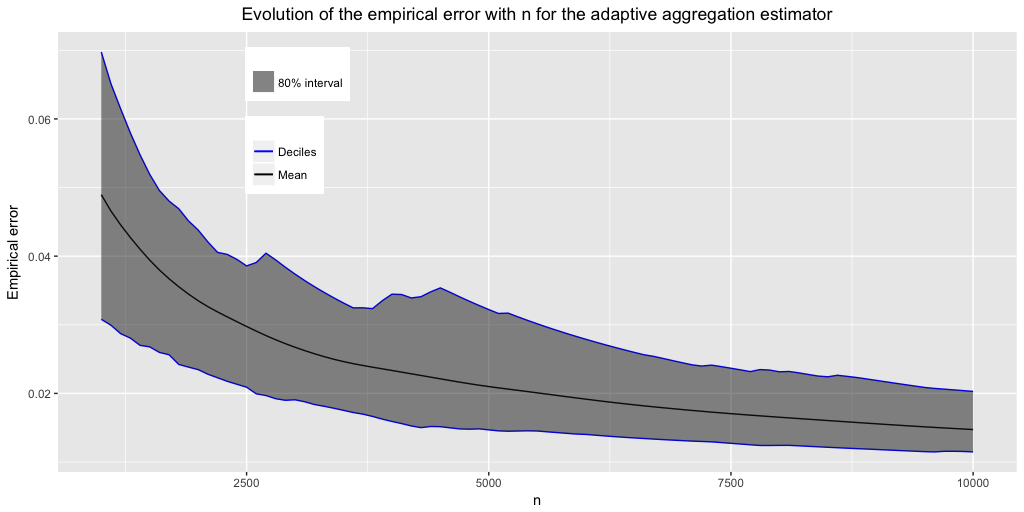
\includegraphics[width=.4\linewidth]{gauss/MCMC/evolution_error_aggregation.png} \\[\abovecaptionskip]
  \end{tabular}
  \begin{tabular}{@{}c@{}}
    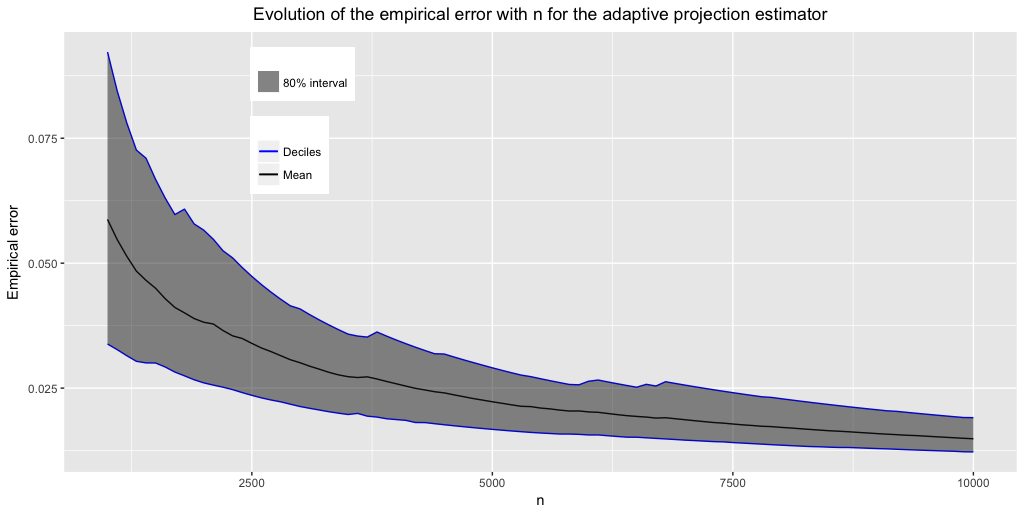
\includegraphics[width=.4\linewidth]{gauss/MCMC/evolution_error_model_selection.png} \\[\abovecaptionskip]
  \end{tabular}
  \caption{Estimation of the evolution with $n$ of the error of the aggregation estimator and of the model selection estimator}
  \label{fig:freq:igssm:error:evol}
\end{figure}

\subsubsection{Minimax optimality}
We now give interest to the maximal risk over Sobolev's ellipsoids.
We aim to apply \nref{ak:ag:ub:pnp:mm} which allows to show that the sequences defined hereafter are upper bounds for the maximal risk of our estimators.
\begin{de*}
  Let be the following family of sequences,
  $\daRa{\Di}{(\xdfCw[])}:=\daRa{\Di}{(\xdfCw[],\Lambda)}:=[\xdfCw^2\vee \DipenSv\,\ssY^{-1}]$.
Considering the following specific case, we aim to show that it describes an upper bound for the maximal risk over $\rwCxdf$ for our aggregation estimator,
    $\aDi{\ssY}(\xdfCw[]):=\argmin\Nset[\Di\in\Nz]{\daRa{\Di}{(\xdfCw[],\Lambda)}}\in\nset{1,\ssY}$\\
    $\naRa{(\xdfCw[])}:=\naRa{(\xdfCw[],\Lambda)}:=\min\Nset[\Di\in\Nz]{\daRa{\Di}{(\xdfCw[],\Lambda)}}$
    with $\daRa{\aDi{\ssY}(\xdfCw[])}{(\xdfCw[],\Lambda)}=\naRa{(\xdfCw[],\Lambda)}$
\assEnd
\end{de*}

The hypotheses to apply \nref{ak:ag:ub:pnp:mm} are the same as for \nref{freq:ge:strat:kn:qu:pnp} and hence we directly obtain the following result.

\begin{thm}
Assume that \nref{freq:ge:strat:kn:qu:as} holds true and consider the penalty sequence $\penSv:=\penD$, $\Di\in\nset{1,n}$, as in \nref{freq:ge:shape:kn:de:pen:oo}.
Let $\txdfAg[{\erWe[]}]=\sum_{\Di=1}^{\ssY} \We\txdfPr$ be an aggregation of the orthogonal series estimators using either aggregation weights $\rWe[]$ as in \eqref{freq:ge:shape:kn:we} or model selection weights $\msWe[]$ as in \eqref{freq:ge:shape:uk:we}. % Let $\Di_{\edf,\xdfCr}:=\floor{3(800\Vnorm[{\xdfCw[]}]{\edf}\xdfCr)^2}$ and
    % $ \ssY_{o}:=15({300})^4$.
There is a finite constant $\cst{\xdfCw[],\xdfCr,\Lambda}$ given in
\eqref{ak:ag:ub:pnp:p8} depending only on $\xdfCw[]$, $\xdfCr$ and $\Lambda$ such that for all
$\ssY\in\Nz$ and for all $\sDi{\ssY}\in\nset{\aDi{\ssY}(\xdfCw[]),\ssY}$  with
 $\aDi{\ssY}(\xdfCw[])\in\nset{1,n}$ as in \nref{freq:ge:strat:kn:ma:de:rate} holds 
 \begin{equation}
 \nRi{\txdfAg[{\erWe[]}]}{\rwCxdf,\Lambda}
   %\sup_{\xdf\in\rwCxdf}\E\Vnormlp{\txdfAg[{\erWe[]}]-\xdf}^2% \leq
    \leq 
   \cst{}(\xdfCr^2\vee1)\min_{\Di\in\nset{1,\ssY}}\big[\daRa{\Di}{(\xdfCw[],\Lambda)}\vee\exp\big(-2\cmiSv\Di\big)]\big)\big]
   +\cst{\xdfCw[],\xdfCr,\Lambda}\ssY^{-1}.
\end{equation}
\reEnd
\end{thm}

\begin{cor}
  Let the assumptions of \nref{ak:ag:ub:pnp:mm} be satisfied.  If in
  addition
  \begin{inparaenum}\item[{{\dgrau\bfseries(A)}}]
    there is $\ssY_{\xdfCw[],\xdfCr,\Lambda}\in\Nz$  such that
    $\aDi{\ssY}({\xdfCw[]})\cmSv[\aDi{\ssY}({\xdfCw[]})]\geq \vert \log\naRa{(\xdfCw[])} \vert/2 $
    for all $\ssY\geq \ssY_{\xdfCw[],\xdfCr,\Lambda}$
  \end{inparaenum}
  holds true, then there is a constant $\cst{\xdfCw[],\xdfCr,\Lambda}$
  depending only on $\rwCxdf$ and $\Lambda$ such that
  $ \nRi{\txdfAg[{\erWe[]}]}{\rwCxdf,\Lambda} \leq
  \cst{\xdfCw[],\xdfCr,\Lambda}\naRa{(\xdfCw[],\Lambda)}$ for all $n\in\Nz$
  holds true.
  \reEnd
\end{cor}


\subsection{Unknown operator}\label{freq:igssm:uk}
We now consider the case when $\lambda$ is unknown and we hence use the observations $(\epsilon_{p})_{p \in \llbracket 1, n_{\lambda} \rrbracket}$ to estimate it.
\subsubsection{Shape of the estimator}
\begin{de*}
We use, as usual an aggregation estimator, where, this time, the aggregating sequence does not depend on $\lambda$ but on $\epsilon^{n_{\lambda}}$,
\begin{equation*}
(\widehat{\theta}^{(\eta)}(s))_{s \in \mathds{F}} = (\sum\nolimits_{m \in \N} \widehat{\P}_{M}^{(\eta)} \cdot \theta_{n, n_{\lambda}, \overline{m}}(s))_{s \in \mathds{F}} = (\sum\nolimits_{m \geq \vert s \vert} \widehat{\P}_{M}^{(\eta)} \cdot \theta_{n, n_{\lambda}}(s))_{s \in \mathds{F}}.
\end{equation*}
In particular, we give the following shape to the aggregating sequence with the contrast $\Upsilon$ and penalty $\pen^{\widehat{\Lambda}}$,
\begin{multline*}
\Upsilon : \N \to \R_{+}, \quad m \mapsto \Upsilon(m); \qquad \pen^{\widehat{\Lambda}} : \N \to \R_{-}, \quad m \mapsto \pen^{\widehat{\Lambda}}(m);\\
\widehat{\P}_{M}^{(\eta)} : \N \to \R_{+}; \quad m \mapsto \tfrac{\exp[\eta n (\Upsilon(m) + \pen^{\widehat{\Lambda}}(m))]}{\sum\nolimits_{k = 0}^{n} \exp[\eta n (\Upsilon(k) + \pen^{\widehat{\Lambda}}(k))]} \mathds{1}_{m \leq n}.
\end{multline*}
Notice that if we let $\eta$ tend to infinity we obtain the following penalised contrast model selection estimator,
\begin{equation*}
  \hDi:=\argmin_{\Di\in\nset{1,\ssY}} \big\{\Upsilon(m)+\peneSv\big\}
\end{equation*}
which corresponds to the following weight sequence,
\begin{equation*}
  \lim_{\rWc\to\infty}\erWe=\dirac[\hDi](\{\Di\})=:\widehat{\P}_{M}^{(\infty)}.
\end{equation*}
In particular, we take the following expressions for $\Upsilon$ and $\pen^{\widehat{\Lambda}}$, with $\kappa := 84$,
\begin{alignat*}{4}
  & \Upsilon(m) && := && \Vert \theta_{n, n_{\lambda}, \overline{m}}\Vert_{l^{2}}^{2}; && \quad \eiSv[(s)]:= \vert \hfedfmpI[(s)] \vert ^2\\
    & \meiSv && := && \max\{\eiSv[(l)],l\in\nset{1,\Di}\}; && \quad \cmeiSv:=\tfrac{\log^{2}(\Di\meiSv\vee(\Di+2))}{\log^{2}(\Di+2)}\geq1;\\
    &\DipeneSv && := && \cmeiSv \Di \meiSv;&& \quad \peneSv:= \peneD.
  \end{alignat*}
\assEnd
\end{de*}

\subsubsection{Oracle optimality}
We first look at the quadratic risk for each $\theta^{\circ}$ and we recall the sequence which shall be an upper bound for the quadratic risk of our estimators.
\begin{de*}
Remind that we defined for any $\theta$ in $\Theta$ and $\Di$ in $\N$ the following term $\b_{m}^{2}(\theta) = \Vert \theta_{\underline{m}} \Vert_{l^{2}}/\Vert \theta_{\underline{0}} \Vert_{l^{2}} \leq 1$.
We then define a family of sequences $(\daRa{\Di}{(\xdf)})_{\Di \in \N} := (\daRa{\Di}{(\xdf,\Lambda)})_{\Di \in \N} = [\b_{m}^{2}(\theta^{\circ}) \vee \penSv/\cpen]$.
We intend to prove that the specific choice
\begin{multline*}
\aDi{\ssY}(\xdf):=\argmin\Nset[\Di\in\Nz]{\daRa{\Di}{(\xdf)}}\in\nset{1,\ssY}; \\
\naRa{(\xdf)}:=\naRa{(\xdf,\Lambda)}:=\min\Nset[\Di\in\Nz]{\daRa{\Di}{(\xdf)}}
\end{multline*}
with $\daRa{\aDi{\ssY}}{(\xdf,\Lambda)}=\naRa{(\xdf,\Lambda)}$ defines an upper bound for the convergence rate of the aggregation estimators.
\assEnd
\end{de*}
Our method gives us a simple assumption to verify in order to obtain this result.

The following result, which is a direct application, once again, of \nref{lmA.1.1} and \nref{lmA.1.2} gives us precisely what we want.
\begin{cor*}
For any $m$, $\ssY$, and $\ssE$ in $\N$ we have,
\begin{alignat*}{3}
& \E_{\phi_{n} \vert \lambda_{n_{\lambda}}}[(\Vert \theta_{n, n_{\lambda}, \overline{m}} - \dxdfPr \Vert_{l^{2}}^{2} - 12 \Delta_{\widehat{\Lambda}}(m) n ^{-1})_{+}] && \leq && 6 n^{-1} \widehat{\Lambda}_{+}(m) \exp[- 2 \delta_{\widehat{\Lambda}}(m)];\\
& \P_{\phi_{n} \vert \lambda_{n_{\lambda}}}[\Vert \theta_{n, n_{\lambda}, \overline{m}} - \dxdfPr \Vert_{l^{2}}^{2} \geq 12 \Delta_{\widehat{\Lambda}}(m) n ^{-1}] && \leq && \exp[- 2 \delta_{\widehat{\Lambda}}(m)];\\
& \P(\vert \lambda_{n_{\lambda}}(s)/\lambda(s) - 1 \vert > 1/3) && \leq && \exp[-\tfrac{n_{\lambda}}{6 \Lambda(s)}].
\end{alignat*}
\reEnd
\end{cor*}

The following theorem is then a direct consequence of \nref{au:ag:ub:pnp} and we omit its proof.
\begin{thm}
Consider the   penalty sequence $\peneSv:=\peneD$,
  $\Di\in\nset{1,\ssY}$, as in \nref{freq:ge:shape:uk:de:pen:oo}.
  Let $\hxdfAg[{\erWe[]}]=\sum_{\Di=1}^{\ssY} \erWe\hxdfPr$ be an aggregation of the orthogonal series estimators using either aggregation weights $\erWe[]$ as in \eqref{freq:ge:shape:uk:we} or model selection weights $\msWe[]$ as in \nref{freq:ge:shape:uk:de:msWe}.
  \begin{Liste}[]
  \item[{\dgrau\bfseries{(p)}}]Assume there is
    $K\in\Nz_0$ with $1\geq \bias[{[K-1] }](\xdf)>0$ and
    $\bias[\Di](\xdf)=0$. For $K>0$ let
    $c_{\xdf}:=\tfrac{\Vnormlp{\xdf_{\underline{0}}}^2+104\cpen}{\Vnormlp{\xdf_{\underline{0}}}^2\bias[{[K-1]}]^2(\xdf)}>1$,
    $\ssY_{\xdf,\Lambda}:=\floor{c_{\xdf}\DipenSv[K]}\in\Nz$ and
    $\ssE(\xdf,\Lambda):=\floor{289\log(K+2)\cmiSv[K]\miSv[K]}\in\Nz$. If
    $\ssY>\ssY_{\xdf,\Lambda}$ and $\ssE>\ssE(\xdf,\Lambda)$ then set
    $\sDi{\ssY}:=\max\{\Di\in\nset{K,\ssY}:\ssY>c_{\xdf}\DipenSv\}$
    and
    $\sDi{\ssE}:=\max\{\Di\in\nset{K,\ssE}:289\log(\Di+2)\cmiSv[\Di]\miSv[\Di]\leq\ssE\}$
    where the defining set, respectively, contains $K$ and thus is not
    empty, and otherwise $\sDi{\ssY}\wedge\sDi{\ssE}:=\Di_{\cst{3}}\log(\ssY\wedge\ssE)$.
    There is a numerical constant $\cst{}$ and a  constant $\cst{\xdf,\Lambda}$ given in
    \eqref{au:ag:ub:pnp:p9} depending only on $\xdf$ and $\Lambda$ such
    that for all $\ssY,\ssE\in\Nz$ holds
    \begin{equation}
       \nmRi{\hxdfAg[{\erWe[]}]}{\xdf,\Lambda}
       %\E\Vnormlp{\widehat{\theta}^{(\eta)}-\xdf}^2
       \leq
      \cst{}\Vnormlp{\xdf_{\underline{0}}}^2\big[\ssY^{-1}\vee \ssE^{-1} \vee
      \exp\big(\tfrac{-\cmiSv[\sDi{\ssY}\wedge\sDi{\ssE}]\sDi{\ssY}\wedge\sDi{\ssE}}{\Di_{\cst{3}}}\big)\big]\\
      + \cst{\xdf,\Lambda}\{\ssY^{-1}\vee\ssE^{-1}\}.
    \end{equation}
  \item[{\dgrau\bfseries{(np)}}] Assume that
    $\bias(\xdf)>0$ for all $\Di\in\Nz$. Let    
    $\ssE(\Lambda):=\floor{289\log(3)\cmiSv[1]\miSv[1]}\in\Nz$. If
    $\ssE>\ssE(\Lambda)$ then set
    $\sDi{\ssE}:=\max\{\Di\in\nset{1,\ssE}:289\log(\Di+2)\cmiSv[\Di]\miSv[\Di]\leq\ssE\}$
    where the defining set, respectively, contains $1$ and thus is not
    empty.  There is a numerical constant $\cst{}$  such that for all $\ssY\in\Nz$
    with $\aDi{\ssY}:=\aDi{\ssY}(\xdf)\in\nset{1,n}$ as in \nref{freq:ge:strat:kn:ma:de:rate} and
    for all $\ssE>\ssE(\Lambda)$ holds
    \begin{multline}
     \nmRi{\hxdfAg[{\erWe[]}]}{\xdf,\Lambda}  
     %\E\Vnormlp{\widehat{\theta}^{(\eta)}-\xdf}^2
     \leq\cst{}(1\vee\Vnormlp{\xdf_{\underline{0}}}^2)\min_{\Di\in\nset{1,\ssY}}\{\daRa{\Di}{(\xdf,\Lambda)}\vee\exp\big(\tfrac{-\cmiSv[\Di]\Di}{\Di_{\cst{3}}}\big)\}\Ind{\{\ssE>\ssE(\Lambda)\}}\\\hfill
+\cst{}(1\vee\Vnormlp{\xdf_{\underline{0}}}^2)\{\bias[\aDi{\ssY}\wedge\sDi{\ssE}]^2(\xdf)\vee\exp\big(\tfrac{-\cmiSv[\sDi{\ssE}]\sDi{\ssE}}{\Di_{\cst{3}}}\big)\}\Ind{\{\ssE>\ssE(\Lambda)\}} \\\hfill
 +\cst{}\mRa{\xdf,\Lambda}   + \cst{}(1\vee\Vnormlp{\xdf_{\underline{0}}}^2)\miSv[1]^2\ssE^{-1}  
    +\cst{}\{\miSv[\Di_{\cst{3}}]^2\Di_{\cst{3}}^3+\miSv[\ssY_{o}]^2\}\ssY^{-1}
  \end{multline}
  while for $\ssE\in\nset{1,\ssE(\Lambda)}$ we have
  
  $\cst{}\mRa{\xdf,\Lambda}
    + \cst{}(1\vee\Vnormlp{\xdf_{\underline{0}}}^2)\miSv[1]^2\ssE^{-1}  
    +\cst{}\{\miSv[\Di_{\cst{3}}]^2\Di_{\cst{3}}^3+\miSv[\ssY_{o}]^2\}\ssY^{-1}$. 
\end{Liste}  
\reEnd
\end{thm}

\begin{cor}
  \begin{Liste}[]
  \item[{\dgrau\bfseries{(p)}}]
    If \ref{ge:ak:ag:ub2:pnp:pc} as in \nref{ge:ak:ag:ub2:pnp} and 
    in addition
    \begin{inparaenum}% \item[\mylabel{ge:au:ag:ub2:pnp:pc:a}{{\dgrau\bfseries(A1)}}]
      % there is $\ssY_{\xdf,\Lambda}\in\Nz$ such that
      % $\cmiSv[\sDi{\ssY}]\sDi{\ssY}\geq \Di_{\cst{3}}(\log\ssY)$ for all
      % $\ssY\geq \ssY_{\xdf,\Lambda}$ and
    \item[{{\dgrau\bfseries(A4)}}]
            there is
            
            $\ssE(\xdf,\Lambda)\in\Nz$ such that
      $\cmiSv[\sDi{\ssE}]\sDi{\ssE}\geq \Di_{\cst{3}}(\log\ssE)$ for all
      $\ssE\geq \ssE(\xdf,\Lambda)$ 
    \end{inparaenum}
    hold true, then there is a constant $\cst{\xdf,\Lambda}$ depending
    only on $\xdf$ and $\Lambda$ such that for all $\ssY,\ssE\in\Nz$ holds
    $\nmRi{\hxdfAg[{\erWe[]}]}{\xdf,\Lambda} \leq
    \cst{\xdf,\Lambda}[\ssY^{-1}\vee\ssE^{-1}]$.
  \item[{\dgrau\bfseries{(np)}}]
    If  \ref{ge:ak:ag:ub2:pnp:npc} as in \nref{ge:ak:ag:ub2:pnp} and \ref{ge:au:ag:ub2:pnp:pc:b}
    hold true, then there is a constant $\cst{\xdf,\Lambda}$ depending
    only on $\xdf$ and $\Lambda$ such that $\nmRi{\hxdfAg[{\erWe[]}]}{\xdf,\Lambda}
    \leq \cst{\xdf,\Lambda}\{\naRa{(\xdf,\Lambda)}+\mRa{\xdf,\Lambda}+\bias[\sDi{\ssE}\wedge\aDi{\ssY}]^2(\xdf)\}$ for all $\ssY,\ssE\in\Nz$ holds true.
  \end{Liste}  
\end{cor}
\subsubsection{Minimax optimality}
We now give interest to the maximal risk over Sobolev's ellipsoids.
We aim to apply \nref{ak:ag:ub:pnp:mm} which allows to show that the sequences defined hereafter are upper bounds for the maximal risk of our estimators.
\begin{de*}
  Let be the following family of sequences,
  $\daRa{\Di}{(\xdfCw[])}:=\daRa{\Di}{(\xdfCw[],\Lambda)}:=[\xdfCw^2\vee \DipenSv\,\ssY^{-1}]$.
Considering the following specific case, we aim to show that it describes an upper bound for the maximal risk over $\rwCxdf$ for our aggregation estimator,
    $\aDi{\ssY}(\xdfCw[]):=\argmin\Nset[\Di\in\Nz]{\daRa{\Di}{(\xdfCw[],\Lambda)}}\in\nset{1,\ssY}$\\
    $\naRa{(\xdfCw[])}:=\naRa{(\xdfCw[],\Lambda)}:=\min\Nset[\Di\in\Nz]{\daRa{\Di}{(\xdfCw[],\Lambda)}}$
    with $\daRa{\aDi{\ssY}(\xdfCw[])}{(\xdfCw[],\Lambda)}=\naRa{(\xdfCw[],\Lambda)}$
\assEnd
\end{de*}

The hypotheses to apply \nref{ak:ag:ub:pnp:mm} are the same as for \nref{freq:ge:strat:kn:qu:pnp} and hence we directly obtain the following result.

\begin{thm}
  Consider the   penalty sequence $\peneSv:=\peneD$,
  $\Di\in\nset{1,\ssY}$, as in \nref{freq:ge:shape:uk:de:pen:oo} with numerical
  constant $\cpen\geq84$. Let
  $\hxdfAg[{\erWe[]}]=\sum_{\Di=1}^{\ssY} \erWe\hxdfPr$ be an
  aggregation of the orthogonal series estimators using either
  aggregation weights $\erWe[]$ as in \eqref{freq:ge:shape:uk:we} or model
  selection weights $\msWe[]$ as in \nref{freq:ge:shape:uk:de:msWe}. Let
  $\dr\Di_{\edf,\xdfCr}:=\floor{3(400\Vnorm[{\xdfCw[]}]{\edf}\xdfCr)^2}$
  and $\dr \ssY_{o}:=15({600})^4$. Let
  $\ssE(\Lambda):=\floor{289\log(3)\cmiSv[1]\miSv[1]}\in\Nz$. If
  $\ssE>\ssE(\Lambda)$ then set
  $\sDi{\ssE}:=\max\{\Di\in\nset{1,\ssE}:289\log(\Di+2)\cmiSv[\Di]\miSv[\Di]\leq\ssE\}$
  where the defining set, respectively, contains $1$ and thus is not
  empty.  There is a numerical constant $\cst{}$ such that for all
  $\ssY\in\Nz$ with $\aDi{\ssY}:=\aDi{\ssY}(\xdf)\in\nset{1,n}$ as in
  \nref{freq:ge:shape:uk:de:pen:oo} and for all $\ssE>\ssE(\Lambda)$ holds
  \begin{multline}
    \nmRi{\hxdfAg[{\erWe[]}]}{\rwCxdf,\Lambda}  
    \leq\cst{}(1\vee\xdfCr^2)\min_{\Di\in\nset{1,\ssY}}
    \{\daRa{\Di}{(\xdfCw[],\Lambda)}\vee
    \exp\big(\tfrac{-\cmiSv[\Di]\Di}{\Di_{\edf,\xdfCr}}\big)\} \\\hfill
    +\cst{}(1\vee\xdfCr^2)\{\xdfCw[(\aDi{\ssY}\wedge\sDi{\ssE})]^2\vee
    \exp\big(\tfrac{-\cmiSv[\sDi{\ssE}]\sDi{\ssE}}{\Di_{\edf,\xdfCr}}\big)\}\\\hfill
    +\cst{}\xdfCr^2\mmRa{\xdfCw[],\Lambda}   + \cst{}(1\vee\xdfCr^2)\miSv[1]^2\ssE^{-1}  
    +\cst{}\{\miSv[\Di_{\edf,\xdfCr}]^2\Di_{\edf,\xdfCr}^3+\miSv[\ssY_{o}]^2\}\ssY^{-1}
  \end{multline}
  while for $\ssE\in\nset{1,\ssE(\Lambda)}$ we have
  \begin{multline}
    \nmRi{\hxdfAg[{\erWe[]}]}{\rwCxdf,\Lambda}  
    \leq \cst{}\xdfCr^2\mmRa{\xdfCw[],\Lambda}
    + \cst{}(1\vee\xdfCr^2)\miSv[1]^2\ssE^{-1}\\
    +\cst{}\{\miSv[\Di_{\edf,\xdfCr}]^2\Di_{\edf,\xdfCr}^3+\miSv[\ssY_{o}]^2\}\ssY^{-1}.
  \end{multline}
\end{thm}


\begin{cor}
  Let the assumptions of \nref{au:mrb:ag:ub:pnp} be satisfied.
    If  \ref{ge:ak:ag:ub2:pnp:npc} as in \nref{ge:ak:ag:ub2:pnp} and \ref{ge:au:ag:ub2:pnp:pc:b}
    as in \nref{ge:au:ag:ub2:pnp} hold true, then there is a constant $\cst{\xdfCw[],\xdfCr,\Lambda}$ depending
    only on $\xdfCw[]$, $\xdfCr$ and $\Lambda$ such that $\nmRi{\hxdfAg[{\erWe[]}]}{\rwCxdf,\Lambda}
    \leq \cst{\xdfCw[],\xdfCr,\Lambda}\{\naRa{(\xdfCw[],\Lambda)}+\mmRa{\xdfCw[],\Lambda}+\xdfCw[(\sDi{\ssE}\wedge\aDi{\ssY})]^2\}$ for all $\ssY,\ssE\in\Nz$ holds true.
\end{cor}